\section{Testing}
\label{sec:testing}
\lhead{\thesection \space Testing}

TODO Marco

\subsection{Quality Management}
\label{ssec:quality_management}

This subsection documents the necessary information required to effectively manage project quality from project planning to delivery. It defines a project’s quality roles, responsibilities, tools, procedures and authorities.

\subsubsection{Plan Quality Management}
\label{ssec:plan_quality}

To ensure a sufficient quality level, every member of the team is involved in the quality process sharing responsibilities. The product owner is involved by providing the test framework.

\begin{table}[H]
    \centering
    \begin{tabular}{|c|c|l|}
        \hline
        \cellcolor{gray}Name & 
        \cellcolor{gray}Role &
        \cellcolor{gray}Responsibilities \\ \hline
        Guido Budziak & Product owner & - Quality mentoring and coaching.\\ \hline
        Lucas Gehlen&Team member&- Taking part in code reviews.\\
        Marco Kull&&- Quality audits.\\
        Patrick Richter&&- Doing manual GUI testing.\\
        Sebastian Wilczek && \\ \hline
    \end{tabular}
    \caption{Quality Roles \& Responsibilities}
    \label{tab:quality_roles}
\end{table}

\subsubsection{Perform Quality Assurance}
\label{ssec:perform_quality}

How the quality test will be performed depends on the type of the module being tested.\\
Design fragments and frontend modules are reviewed and, in case of front end modules, manually tested. They are then presented and discussed by the whole team and the product owner at the weekly meetings.\\

\subsubsection{Control Quality}
\label{ssec:control_quality}

\begin{figure}[H]
    \begin{center}
        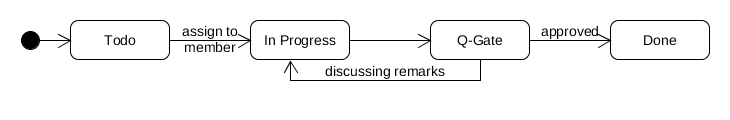
\includegraphics[width=0.9\textwidth]{images/state-quality.png}
        \caption{Quality Process}
        \label{fig:quality_process}
    \end{center}
\end{figure}

To ensure complete quality testing on the software every completed part will be assigned to a quality testing state. A team member that has not been part of the creation of the relevant piece then performs the quality testing.

\subsection{Requirements Quality Check}
\label{ssec:requirements_quality_check}

TODO Marco

\subsection{Deployment \& Manual Testing}
\label{ssec:deployment_manual_testing}

TODO Marco

\subsection{Testing \textit{React Native}}
\label{ssec:testing_react_native}

Like any software product, \textit{React Native} applications have to be tested for proper functionality and stability. As mentioned in \textit{\ref{ssec:deployment_manual_testing} \nameref{ssec:deployment_manual_testing}}, testing in this project was mainly done by simulating use cases and testing new functionality by hand, inputting values and user interaction into a deployed version of the application.
\newline
The manual testing approach was mostly taken since the existing base of the application proved to be largely incompatible. \textit{Appendix \ref{appendix:research_paper_sebastian_wilczek}: \nameref{appendix:research_paper_sebastian_wilczek}} contains a research paper detailing different testing frameworks and environments for \textit{React Native}, including usage examples and descriptions as to why they are incompatible or hard to use with the application in question.
\newline
Theoretically though, if the application did not show as many problems with existing testing frameworks, testing could be made more efficient by writing automatic end-to-end tests. One framework that can be made use of to write such tests is \textit{Appium}. Listing \ref{lst:appium_test} shows a test written \textit{WebdriverIO} in combination with \textit{Appium} that tests the application.

\begin{lstlisting}[language=javascript, caption=\textit{Appium} end-to-end test, label=lst:appium_test]
const webdriverio = require("webdriverio");
const opts = {
  port: 4723,
  desiredCapabilities: {
    platformName: "Android",
    platformVersion: "9",
    deviceName: "Nexus 5X API 28 x86",
    app: "[...]/SoFa/android/app/build/outputs/apk/debug/app-debug.apk",
    automationName: "UiAutomator2"
  }
};
describe("Basic Android interactions", function() {
  let client;
  beforeEach(function() {
    client = webdriverio.remote(opts);
    return client.init().pause(15000);
  });
  afterEach(function() {
    return client.end();
  });
  it("should click a tab that opens more functionality", async function() {
    return client
      .waitForExist('~More', 5000)
      .element('~More')
      .click()
      .waitForExist("~Privacy", 5000)
      .getText("~Privacy", function(result) {
        assert.equal(result.value, "Privacy");
      });
  });
});
\end{lstlisting}

The test is constructed relatively simple. It is first defined on what platform the test is supposed to be ran. In this case, it is an \textit{Android} device with the identification "Nexus 5X API 28 x86", which is the emulator running on the development machine. Furthermore, a path is given to an "apk" file, which is the build file of the application itself, telling the test that this is the application to be tested.
\newline
The actual tests are defined afterwards. In this example, the driver, which is \textit{WebdriverIO}, is supposed to connect to the emulator before each test and to disconnect afterwards. The test itself waits for an element with the \textit{Accessibility Label} "More" to exists, clicks that element, waits for another one with the value "Privacy", and finally checks if that component has the text value "Privacy". This is a simple test to see if the main screen of the application can switch between tabs. This test fails due to incompatibility reasons. For further information see the research paper mentioned at the beginning of this section.
\newline
Single \textit{React Native} components can also be tested using \textit{Jest}, which creates snapshots of component rendering and compares them each time the tests are ran. If there is a change in the rendering, the change is marked and the developer can decide whether the change is intentional or an error. If it is intentional, the snapshot is overwritten so it can be used during the next test.
\newline
However, \textit{Jest} is also largely unusable during this project. The nature of \textit{Jest} makes it more applicable to unit tests. Furthermore, since most of the newly developed components are functional components, \textit{Jest} also is unable to create snapshots, which means that these components can only be tested if they are first wrapped in non-functional components. This is a lot of extra work for the developers and is ultimately not worth it.